
%% Paper.tex
%% V1.4b
%% 2017/05/17
%% by jyc
%% See:
%%
%% This is a skeleton file demonstrating the use of IEEEtran.cls
%% (requires IEEEtran.cls version 1.8b or later) with an IEEE
%% conference paper.
%%
%% Support sites:
%% http://www.michaelshell.org/tex/ieeetran/
%% http://www.ctan.org/pkg/ieeetran
%% and
%% http://www.ieee.org/

%%*************************************************************************
%% Legal Notice:
%% This code is offered as-is without any warranty either expressed or
%% implied; without even the implied warranty of MERCHANTABILITY or
%% FITNESS FOR A PARTICULAR PURPOSE! 
%% User assumes all risk.
%% In no event shall the IEEE or any contributor to this code be liable for
%% any damages or losses, including, but not limited to, incidental,
%% consequential, or any other damages, resulting from the use or misuse
%% of any information contained here.
%%
%% All comments are the opinions of their respective authors and are not
%% necessarily endorsed by the IEEE.
%%
%% This work is distributed under the LaTeX Project Public License (LPPL)
%% ( http://www.latex-project.org/ ) version 1.3, and may be freely used,
%% distributed and modified. A copy of the LPPL, version 1.3, is included
%% in the base LaTeX documentation of all distributions of LaTeX released
%% 2003/12/01 or later.
%% Retain all contribution notices and credits.
%% ** Modified files should be clearly indicated as such, including  **
%% ** renaming them and changing author support contact information. **
%%*************************************************************************


% *** Authors should verify (and, if needed, correct) their LaTeX system  ***
% *** with the testflow diagnostic prior to trusting their LaTeX platform ***
% *** with production work. The IEEE's font choices and paper sizes can   ***
% *** trigger bugs that do not appear when using other class files.       ***                          ***
% The testflow support page is at:
% http://www.michaelshell.org/tex/testflow/



\documentclass[conference]{IEEEtran}
% Some Computer Society conferences also require the compsoc mode option,
% but others use the standard conference format.
%
% If IEEEtran.cls has not been installed into the LaTeX system files,
% manually specify the path to it like:
% \documentclass[conference]{../sty/IEEEtran}



% Some very useful LaTeX packages include:
% (uncomment the ones you want to load)


% *** MISC UTILITY PACKAGES ***
%
%\usepackage{ifpdf}
% Heiko Oberdiek's ifpdf.sty is very useful if you need conditional
% compilation based on whether the output is pdf or dvi.
% usage:
% \ifpdf
%   % pdf code
% \else
%   % dvi code
% \fi
% The latest version of ifpdf.sty can be obtained from:
% http://www.ctan.org/pkg/ifpdf
% Also, note that IEEEtran.cls V1.7 and later provides a builtin
% \ifCLASSINFOpdf conditional that works the same way.
% When switching from latex to pdflatex and vice-versa, the compiler may
% have to be run twice to clear warning/error messages.






% *** CITATION PACKAGES ***
%
\usepackage{cite}
% cite.sty was written by Donald Arseneau
% V1.6 and later of IEEEtran pre-defines the format of the cite.sty package
% \cite{} output to follow that of the IEEE. Loading the cite package will
% result in citation numbers being automatically sorted and properly
% "compressed/ranged". e.g., [1], [9], [2], [7], [5], [6] without using
% cite.sty will become [1], [2], [5]--[7], [9] using cite.sty. cite.sty's
% \cite will automatically add leading space, if needed. Use cite.sty's
% noadjust option (cite.sty V3.8 and later) if you want to turn this off
% such as if a citation ever needs to be enclosed in parenthesis.
% cite.sty is already installed on most LaTeX systems. Be sure and use
% version 5.0 (2009-03-20) and later if using hyperref.sty.
% The latest version can be obtained at:
% http://www.ctan.org/pkg/cite
% The documentation is contained in the cite.sty file itself.


\usepackage{listings}
\usepackage{graphicx}
\usepackage{xcolor}
\lstset{
    numbers=left, 
    basicstyle=\footnotesize\ttfamily, 
    numberstyle= \tiny, 
    keywordstyle= \color{ blue!70},
    commentstyle= \color{red!50!green!50!blue!50}, 
    numbersep=5pt,   % how far the line-numbers are from the code
    frame=shadowbox, % 阴影效果
    rulesepcolor= \color{ red!20!green!20!blue!20} ,
    escapeinside=``, % 英文分号中可写入中文
    xleftmargin=3em,xrightmargin=2em, aboveskip=1em,
    framexleftmargin=2em
} 

% *** GRAPHICS RELATED PACKAGES ***
%
\ifCLASSINFOpdf
  % \usepackage[pdftex]{graphicx}
  % declare the path(s) where your graphic files are
  % \graphicspath{{../pdf/}{../jpeg/}}
  % and their extensions so you won't have to specify these with
  % every instance of \includegraphics
  % \DeclareGraphicsExtensions{.pdf,.jpeg,.png}
\else
  % or other class option (dvipsone, dvipdf, if not using dvips). graphicx
  % will default to the driver specified in the system graphics.cfg if no
  % driver is specified.
  % \usepackage[dvips]{graphicx}
  % declare the path(s) where your graphic files are
  % \graphicspath{{../eps/}}
  % and their extensions so you won't have to specify these with
  % every instance of \includegraphics
  % \DeclareGraphicsExtensions{.eps}
\fi
% graphicx was written by David Carlisle and Sebastian Rahtz. It is
% required if you want graphics, photos, etc. graphicx.sty is already
% installed on most LaTeX systems. The latest version and documentation
% can be obtained at: 
% http://www.ctan.org/pkg/graphicx
% Another good source of documentation is "Using Imported Graphics in
% LaTeX2e" by Keith Reckdahl which can be found at:
% http://www.ctan.org/pkg/epslatex
%
% latex, and pdflatex in dvi mode, support graphics in encapsulated
% postscript (.eps) format. pdflatex in pdf mode supports graphics
% in .pdf, .jpeg, .png and .mps (metapost) formats. Users should ensure
% that all non-photo figures use a vector format (.eps, .pdf, .mps) and
% not a bitmapped formats (.jpeg, .png). The IEEE frowns on bitmapped formats
% which can result in "jaggedy"/blurry rendering of lines and letters as
% well as large increases in file sizes.
%
% You can find documentation about the pdfTeX application at:
% http://www.tug.org/applications/pdftex





% *** MATH PACKAGES ***
%
%\usepackage{amsmath}
% A popular package from the American Mathematical Society that provides
% many useful and powerful commands for dealing with mathematics.
%
% Note that the amsmath package sets \interdisplaylinepenalty to 10000
% thus preventing page breaks from occurring within multiline equations. Use:
%\interdisplaylinepenalty=2500
% after loading amsmath to restore such page breaks as IEEEtran.cls normally
% does. amsmath.sty is already installed on most LaTeX systems. The latest
% version and documentation can be obtained at:
% http://www.ctan.org/pkg/amsmath





% *** SPECIALIZED LIST PACKAGES ***
%
%\usepackage{algorithmic}
% algorithmic.sty was written by Peter Williams and Rogerio Brito.
% This package provides an algorithmic environment fo describing algorithms.
% You can use the algorithmic environment in-text or within a figure
% environment to provide for a floating algorithm. Do NOT use the algorithm
% floating environment provided by algorithm.sty (by the same authors) or
% algorithm2e.sty (by Christophe Fiorio) as the IEEE does not use dedicated
% algorithm float types and packages that provide these will not provide
% correct IEEE style captions. The latest version and documentation of
% algorithmic.sty can be obtained at:
% http://www.ctan.org/pkg/algorithms
% Also of interest may be the (relatively newer and more customizable)
% algorithmicx.sty package by Szasz Janos:
% http://www.ctan.org/pkg/algorithmicx




% *** ALIGNMENT PACKAGES ***
%
%\usepackage{array}
% Frank Mittelbach's and David Carlisle's array.sty patches and improves
% the standard LaTeX2e array and tabular environments to provide better
% appearance and additional user controls. As the default LaTeX2e table
% generation code is lacking to the point of almost being broken with
% respect to the quality of the end results, all users are strongly
% advised to use an enhanced (at the very least that provided by array.sty)
% set of table tools. array.sty is already installed on most systems. The
% latest version and documentation can be obtained at:
% http://www.ctan.org/pkg/array


% IEEEtran contains the IEEEeqnarray family of commands that can be used to
% generate multiline equations as well as matrices, tables, etc., of high
% quality.




% *** SUBFIGURE PACKAGES ***
%\ifCLASSOPTIONcompsoc
%  \usepackage[caption=false,font=normalsize,labelfont=sf,textfont=sf]{subfig}
%\else
%  \usepackage[caption=false,font=footnotesize]{subfig}
%\fi
% subfig.sty, written by Steven Douglas Cochran, is the modern replacement
% for subfigure.sty, the latter of which is no longer maintained and is
% incompatible with some LaTeX packages including fixltx2e. However,
% subfig.sty requires and automatically loads Axel Sommerfeldt's caption.sty
% which will override IEEEtran.cls' handling of captions and this will result
% in non-IEEE style figure/table captions. To prevent this problem, be sure
% and invoke subfig.sty's "caption=false" package option (available since
% subfig.sty version 1.3, 2005/06/28) as this is will preserve IEEEtran.cls
% handling of captions.
% Note that the Computer Society format requires a larger sans serif font
% than the serif footnote size font used in traditional IEEE formatting
% and thus the need to invoke different subfig.sty package options depending
% on whether compsoc mode has been enabled.
%
% The latest version and documentation of subfig.sty can be obtained at:
% http://www.ctan.org/pkg/subfig




% *** FLOAT PACKAGES ***
%
%\usepackage{fixltx2e}
% fixltx2e, the successor to the earlier fix2col.sty, was written by
% Frank Mittelbach and David Carlisle. This package corrects a few problems
% in the LaTeX2e kernel, the most notable of which is that in current
% LaTeX2e releases, the ordering of single and double column floats is not
% guaranteed to be preserved. Thus, an unpatched LaTeX2e can allow a
% single column figure to be placed prior to an earlier double column
% figure.
% Be aware that LaTeX2e kernels dated 2015 and later have fixltx2e.sty's
% corrections already built into the system in which case a warning will
% be issued if an attempt is made to load fixltx2e.sty as it is no longer
% needed.
% The latest version and documentation can be found at:
% http://www.ctan.org/pkg/fixltx2e


%\usepackage{stfloats}
% stfloats.sty was written by Sigitas Tolusis. This package gives LaTeX2e
% the ability to do double column floats at the bottom of the page as well
% as the top. (e.g., "\begin{figure*}[!b]" is not normally possible in
% LaTeX2e). It also provides a command:
%\fnbelowfloat
% to enable the placement of footnotes below bottom floats (the standard
% LaTeX2e kernel puts them above bottom floats). This is an invasive package
% which rewrites many portions of the LaTeX2e float routines. It may not work
% with other packages that modify the LaTeX2e float routines. The latest
% version and documentation can be obtained at:
% http://www.ctan.org/pkg/stfloats
% Do not use the stfloats baselinefloat ability as the IEEE does not allow
% \baselineskip to stretch. Authors submitting work to the IEEE should note
% that the IEEE rarely uses double column equations and that authors should try
% to avoid such use. Do not be tempted to use the cuted.sty or midfloat.sty
% packages (also by Sigitas Tolusis) as the IEEE does not format its papers in
% such ways.
% Do not attempt to use stfloats with fixltx2e as they are incompatible.
% Instead, use Morten Hogholm'a dblfloatfix which combines the features
% of both fixltx2e and stfloats:
%
% \usepackage{dblfloatfix}
% The latest version can be found at:
% http://www.ctan.org/pkg/dblfloatfix




% *** PDF, URL AND HYPERLINK PACKAGES ***
%
%\usepackage{url}
% url.sty was written by Donald Arseneau. It provides better support for
% handling and breaking URLs. url.sty is already installed on most LaTeX
% systems. The latest version and documentation can be obtained at:
% http://www.ctan.org/pkg/url
% Basically, \url{my_url_here}.




% *** Do not adjust lengths that control margins, column widths, etc. ***
% *** Do not use packages that alter fonts (such as pslatex).         ***
% There should be no need to do such things with IEEEtran.cls V1.6 and later.
% (Unless specifically asked to do so by the journal or conference you plan
% to submit to, of course. )


% correct bad hyphenation here
\hyphenation{op-tical net-works semi-conduc-tor}


\begin{document}
%
% paper title
% Titles are generally capitalized except for words such as a, an, and, as,
% at, but, by, for, in, nor, of, on, or, the, to and up, which are usually
% not capitalized unless they are the first or last word of the title.
% Linebreaks \\ can be used within to get better formatting as desired.
% Do not put math or special symbols in the title.
\title{A flexible parallel architecture for\\ high-performance network traffic processing}


% author names and affiliations
% use a multiple column layout for up to three different
% affiliations
\author{\IEEEauthorblockN{Yanchao Jing}
\IEEEauthorblockA{School of Shanghai\\
Jiao Tong University\\
Email:13541333146@163.com}
\and
\IEEEauthorblockN{Guangtao Xue}
\IEEEauthorblockA{School of Shanghai\\
Jiao Tong University\\
Email: homer@thesimpsons.com}
\and
\IEEEauthorblockN{ShiyouQian}
\IEEEauthorblockA{School of Shanghai\\
Jiao Tong University\\
Email:}}

% conference papers do not typically use \thanks and this command
% is locked out in conference mode. If really needed, such as for
% the acknowledgment of grants, issue a \IEEEoverridecommandlockouts
% after \documentclass

% for over three affiliations, or if they all won't fit within the width
% of the page, use this alternative format:
% 
%\author{\IEEEauthorblockN{Michael Shell\IEEEauthorrefmark{1},
%Homer Simpson\IEEEauthorrefmark{2},
%James Kirk\IEEEauthorrefmark{3}, 
%Montgomery Scott\IEEEauthorrefmark{3} and
%Eldon Tyrell\IEEEauthorrefmark{4}}
%\IEEEauthorblockA{\IEEEauthorrefmark{1}School of Electrical and Computer Engineering\\
%Georgia Institute of Technology,
%Atlanta, Georgia 30332--0250\\ Email: see http://www.michaelshell.org/contact.html}
%\IEEEauthorblockA{\IEEEauthorrefmark{2}Twentieth Century Fox, Springfield, USA\\
%Email: homer@thesimpsons.com}
%\IEEEauthorblockA{\IEEEauthorrefmark{3}Starfleet Academy, San Francisco, California 96678-2391\\
%Telephone: (800) 555--1212, Fax: (888) 555--1212}
%\IEEEauthorblockA{\IEEEauthorrefmark{4}Tyrell Inc., 123 Replicant Street, Los Angeles, California 90210--4321}}




% use for special paper notices
%\IEEEspecialpapernotice{(Invited Paper)}




% make the title area
\maketitle

% As a general rule, do not put math, special symbols or citations
% in the abstract
\begin{abstract}
Nowadays,the deep packet inspection(DPI) becomes a crucial technique to monitor the security of network which needs the completed information of network traffic packets.This technique claim an extremely strict requirement on the functionality and performance of a monitor subsystem.Therefore, a high-performance easy-use network traffic capture library is extremely required to help to build some attractive DPI applications.
\newline\indent To feed this demand,this paper proposes a flexible parallel network library(noff) which has ability to process the network traffic in multiple Gbps speed.With several innovative software techniques,noff has remarkably optimized the packets delivery procedure and the streams reassembly procedure compared with some traditional methods.Supporting two
kinds of parallel processing on multi-core architectures, minimizing memory allocation and dropping silent streams effectively are the main features of noff.Some well-designed experimental evaluations indicate that noff can perform better than other software libraries in streams reassembly and http parser on single core, and can process much higher traffic loads when using multi-core platform.

\end{abstract}

% no keywords




% For peer review papers, you can put extra information on the cover
% page as needed:
% \ifCLASSOPTIONpeerreview
% \begin{center} \bfseries EDICS Category: 3-BBND \end{center}
% \fi
%
% For peerreview papers, this IEEEtran command inserts a page break and
% creates the second title. It will be ignored for other modes.
\IEEEpeerreviewmaketitle



\section{Introduction}
% no \IEEEPARstart
Nowadays the demand for quality of service (Qos) and network security including policy-based routing,firewall and virtual private network(VPN) is ever-increasing\cite{Liu},In order to satisfy the requirement,An in-depth understanding of the Internet traffic profile is needed.Accordingly, the deep packet inspection(DPI) becomes a crucial hot technology\cite{Antonello}.In a nutshell,a DPI system Firstly has to collect packets from the network interface cards(NIC),then to create a data structure to represent the incoming packets as network flows and then to forward or store the received packets for further processing.So it is extremely necessary to capture all exchanged packets between end-systems on the monitored link in very high speed links (e.g. multiple Gbps).\cite{Antonello}.Many DPI applications deeply rely on information from the network packets.Therefore a high-performance easy-use network traffic capture library is extremely required.
\newline\indent Recently, For high-performance,enormous relative theoretical methods and tools have been proposed such as zero-copy technology, multi-core capture,multi-thread method and FPGA tools\cite{Qiao} and so on. This paper mainly focuses on software optimization.
The zero-copy and multi-core technology can help avoid sparse sampling\cite{Ali}.A renowned tool to accomplish zero-copy is PF\_RING\cite{PFRING}\cite{Luca}.The PF\_RING kernel module runs as a software interrupt handler that stores incoming packets to a memory-mapped buffer,shared with user-level stub.For multi-core technology,there are also various multi-thread proposed methods that can improve the entire performance.
The key of multi-thread is to make the best of multi-core performance.
\newline\indent Although there are many kinds of theoretical technologies, there is hardly a flexible high-performance network traffic library. Under such conditions, developing a strong DPI application becomes a huge challenge.
\newline\indent To overcome this difficulty, in this paper we present a parallel network traffic library(noff),a high-performance passive network traffic monitoring framework.Noff provides the high-level functions needed by many monitoring applications and provide a quite flexible framework to adjust the system structure .Application developers can easily create magic high-level applications based on noff.
\newline\indent To acquire aggressive performance optimization, we use a flexible multi-thread structure which can make the best of the multi-core performance to achieve a high throughput.
\newline\indent To reduce the overhead of unnecessary memory copying.Noff uses the PF\_RING as underlying kernel component. The subzero packet copy scheme of PF\_RING can contribute to reduce the total overhead and noff also uses the TCMalloc\cite{Evans}\cite{Sangho} framework to reduce the memory allocation frequency.Meanwhile,noff adopts some novel techniques to reduce the overhead of thread synchronization. 
\newline\indent To accommodate heavy loads, noff introduces the notion of Least Recently Used (LRU) stream management algorithm.Under heavy load,traditional monitoring systems usually drop arriving packets in a random way, which would severely affect the following stream reassembly process.Noff always drop the dead stream which has no data exchange during a long time.This method can relatively reduce the impacts from dropping streams.
\newline\indent Noff also provides a flexible and expressive application programming interface that allows programmers to develop many kinds of interesting traffic applications.Our design introduces two novel features:(\uppercase\expandafter{\romannumeral1}) Noff uses the C++ bind and function features to design callback interfaces between two modules.Programmers can flexibly add new modules or change modules just through main configure file. And(\uppercase\expandafter{\romannumeral2})it offers more control for tolerating packet loss under high load throughput. And noff also supports single queue NIC's multi-thread scaling and multiple queue based on RSS(receive-side scaling)\cite{Server} transparent parallelization of stream processing simultaneously.
\newline\indent We have evaluated noff in a 10GbE environment using real campus traffic and showed that it outperforms existing alternatives like Libnids and Snort's\cite{snort} stream5 processor in a variety of scopes.For example,our results demonstrate that noff can capture and deliver all streams with lower CPU utilization.
The main contributions of this paper are:
\newline 1.We propose noff, which is an universal network traffic library.It provides a flexible and aggressive software framework to offer programmers an easy-use platform to develop network plug-in compartments.
\newline 2.We introduce some applied software techniques to optimize traditional products and approaches.Through these techniques,noff can deliver transport-layer streams for higher traffic rates than previous approaches.
\newline 3.We introduce Least Recently Used (LRU), an innovate algorithm that enables a graceful adaptation to overload conditions by dropping packets of dead streams,and favoring streams that exchange data frequently.

\section{software Feature}
The design of noff focuses attention on two key objectives: structure flexibility and runtime performance.In this part, we introduce the main aspects of software feature of noff across these following six dimensions.

% You must have at least 2 lines in the paragraph with the drop letter
% (should never be an issue)
\subsection{Flexble Module Framework and Interface}

Noff adopts a novel callback module interface which is based on the function template feature of C++. Noff is composed of several modules.
These modules can be structured into several parts according to functionality or logical structure. The logical structure of noff includes capturer,dispatcher,IP,TCP,UDP,application and so on,which is correspond to the TCP/IP network model.Each layer will offer one or more callback interface to many upper layer modules. Programmers can build their modules on lower layer modules without changing any existing code.Furthermore, noff can selectively assemble different modules into a same layer to adapt to different demands.

\subsection{PF\_RING Patch}
PF\_RING is a new type of network socket that can dramatically improve the packet capture speed.It uses User-space ZC (new generation DNA, Direct NIC Access) drivers for extreme packet capture transmission speed as the NIC NPU (Network Process Unit) is pushing getting packets to user land without any kernel intervention. 
Noff uses PF\_RING as the kernel driver and can thus arrive more aggressive runtime speed.

\subsection{LRU Scheme}
Noff has proposed Least Recently Used(LRU):a stream algorithm which enables the system to control its resources effectively during overload. This algorithm can resolve the problem that sudden traffic bursts or overload conditions may force the packet capturing subsystem to fill up its buffers and randomly drop streams in a haphazard manner.In order to arrive this requirment,noff maintains a novel timer data structure:timing wheel\cite{Varghese}which store the streams into different buckets by the time gap.Timing wheel would drop the streams which have been silent for at least one minute.In this way,the new stream will be accommodated with a higher probability.Besides,Programmers can also force to maintain some priority streams by updating the timestamp of those streams.The detail implementation of timing wheel would be described in the implementation section.

\subsection{Flexible Stream Reassembly}
Libnids\cite{Libnids} has accomplished its TCP reassembly machine by simplifying the Linux network stack. However,the callback interface of libnids is a little poor and
it has no ability to cope with the connection abnormity because of none timer. Noff adds a passive keep-alive timer to close the dead abnormal connection when
a stream connection has no data interaction during a long time. Noff also abandons the TCP memory buffer in libnids to reduce memory copy overhead. Besides,noff reserves nearly all of the other functions of libnids.

\subsection{Memory Allocations Optimization}
On the one hand,Noff uses TCMalloc\cite{Threading}\cite{Sangho} to optimize the memory copy performance. The TCMalloc implementation performs better than the traditional tools.TCMalloc assigns each thread a thread-local cache. Small allocations are satisfied from the thread-local cache. when a cache is insufficient,memories are moved from central data structures into the thread-local cache as needed, and periodic garbage collections are used to migrate memory back from a thread-local cache into the central data structures ,which clearly reduce the frequency of memory allocation.
\newline\indent On the other hand,Noff also uses smart pointer to manage objects to enhance the security of memory management.

\subsection{Parallel Processing}
Noff offers two kinds of multi-thread platforms which inherent support for multi-core systems.The two kinds are all achieved by transparently creating a number of worker threads for user-level stream processing the number of those threads is equal to the number the available cores.All processing of a particular stream is done on the same core, reducing,in this way, context switches, cache misses, and interthread synchronization operations.
\newline\indent To balance the network traffic load across multiple NIC queues and cores, Scap\cite{Papadogiannakis} uses kernel based approach such as Receive Side Scaling (RSS)\cite{Server}to process balance a lot number of packets.While,in our implementation,when the NIC supports multiple queue,noff could use RSS to assign one stream to a corresponding thread equably.Otherwise,noff could even use customized load balancer to assign each stream.

\section{Architecture}
This section describes the architecture of the noff framework for capturing and processing.
\subsection{Kernel Capture}
The Capture module of noff has two shapes:the first one mainly support Multiple queue NICs which use a loadable kernel module and a user-level API stub,as shown in Figure \ref{fig:1}. In this case,Noff would initialize several threads which have same number towards NIC queues.
Then PF\_RING kernel module transfers stream packets between queue and thread.
\newline\indent The second one is mainly designed for NICs which only have one receive queue.This case is shown in Figure \ref{fig:2}. Programmer can choose a suitable shapes according to practical situation which Reflects the versatility of our capture module.

\subsection{Processing Procedure}
Noff uses a multi-layer framework. Each layer is independent and could include a number of modules.A module would offer one or more callback interface for upper layer module to invoke. A stream packet's processing procedure is shown as Figure \ref{fig:3}.
Programmer can add a new module based on one existing layer by themselves.
\begin{figure}
\begin{minipage}[t]{0.495\linewidth}
\flushleft
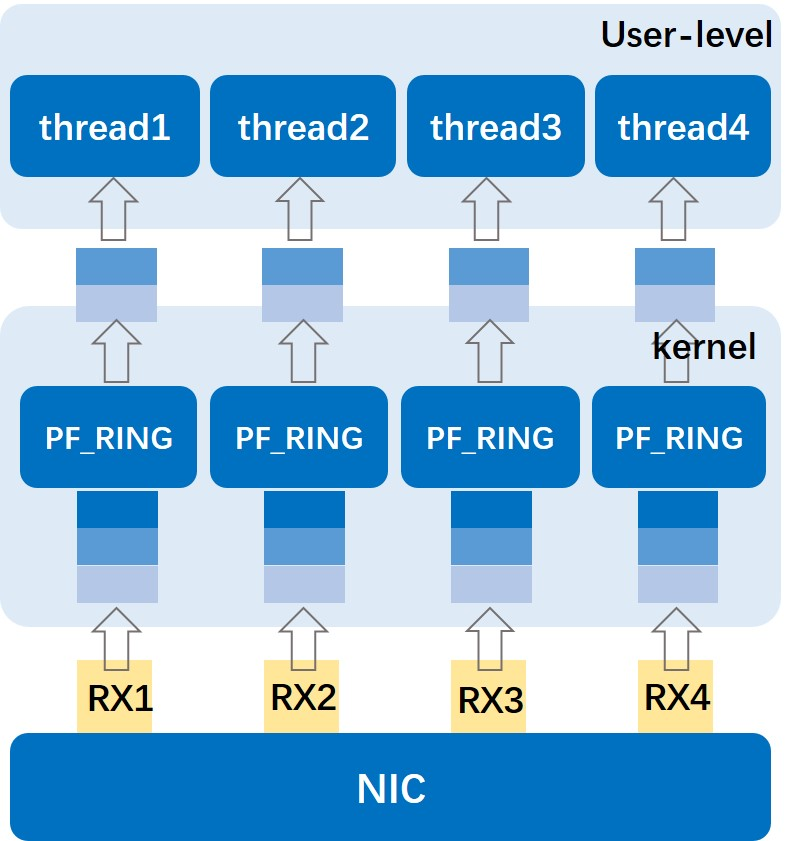
\includegraphics[width=\textwidth]{./picture/Figure1.jpg}
\caption{Multiple Queues Capture} 
\label{fig:1}
\end{minipage}
\begin{minipage}[t]{0.495\linewidth}
\flushright
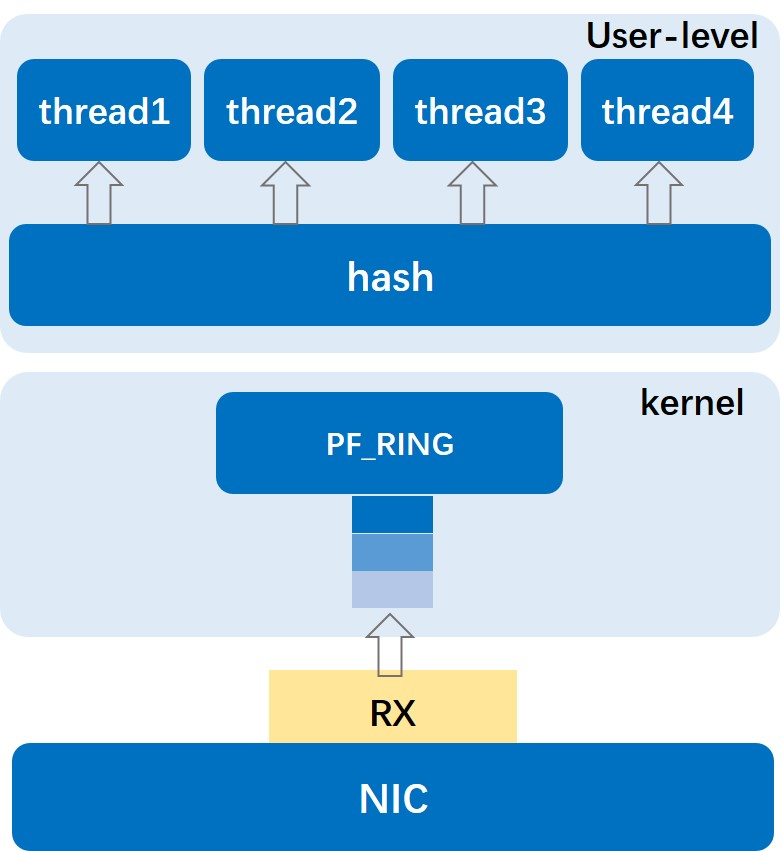
\includegraphics[width=\textwidth]{./picture/Figure2.jpg}
\caption{Single Queue Capture}
\label{fig:2}
\end{minipage}
\end{figure} 

\begin{figure}[htbp]
  \centering
  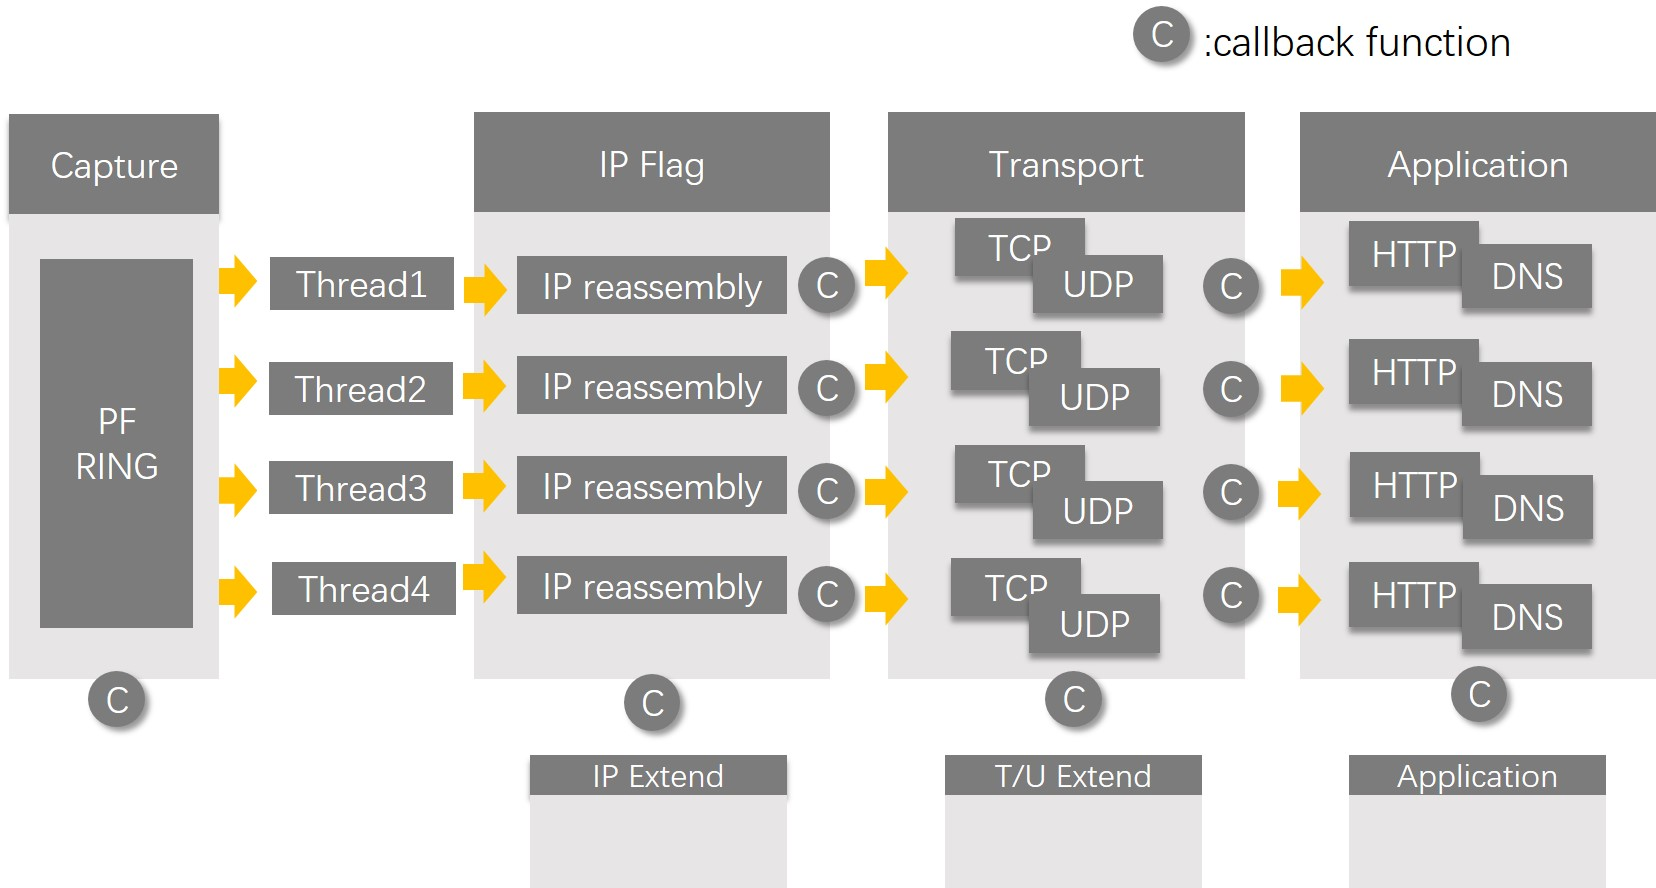
\includegraphics[width=0.5\textwidth]{./picture/Figure3.jpg}
  \caption{Packet Processing Procedure}
  \label{fig:3}
\end{figure}

\section{Noff Modules}
This section describes the module of noff and shows how to build and register a new module.
\subsection{Module Structure}
Noff's module is a C++ class. Each module should be responsible for a corresponding procedure.A module use a public function to invoke another module's interface in lower layer to acquire the necessary data.Meanwhile,this module also needs to offer a callback interface for upper layer modules through the function template feature.For instance, a module class is just simplify shown as Figure \ref{fig:4}. \newline\indent Figure \ref{fig:4} displays the nucleus functions of the capture module. vector$<$PacketCallback$>$ and vector$<$IpFragmentCall$>$ save all of the upper layer callback functions. Because these two vector are all private members. So programers should use \textbf{addPacketCallBack} and \textbf{addIpFragmentCallback} to operate these two private vectors.The \textbf{internalCallback} function is the key interface for lower layer modules to invoke.In conclusion,a valid module of noff should at least include a key interface for lower layer to invoke and at least one callback vector for upper layer modules to register callback function.
\subsection{Module Configuration}
After accomplishing one module,it is necessary to configure this module into the main file. The DNS module configuration is shown as following code block.As noff is a multi-thread platform,so we use the thread local variable to allocate module instance for each thread.Using this method,we need not to consider thread synchronization issues.In a module code block,we need firstly acquire the instance reference.Then we  should register the upper callback interface to callback vector and register the key interface of this module to lower layer module.Finally,we should put our module function into \textbf{initInThread} function. In this way, this new module would work normally.
\begin{lstlisting}[language=C]
void setDnsCounterInThread()
{
    auto& udp = threadInstance(Udp);
    auto& dns = threadInstance(DnsParser);
    udp.addUdpCallback(bind(
    &DnsParser::processDns, &dns, 
    _1, _2, _3, _4));

    dns.addRequstecallback(bind(
    &UdpClient::onData<DnsRequest>,
    dnsRequestOutput.get(), _1));

    dns.addResponsecallback(bind(
    &UdpClient::onData<DnsResponse>,
    dnsResponseOutput.get(), _1));
}
void initInThread()
{
 setDnsCounterInThread();
}
\end{lstlisting}
\begin{figure}[htbp]
  \centering
  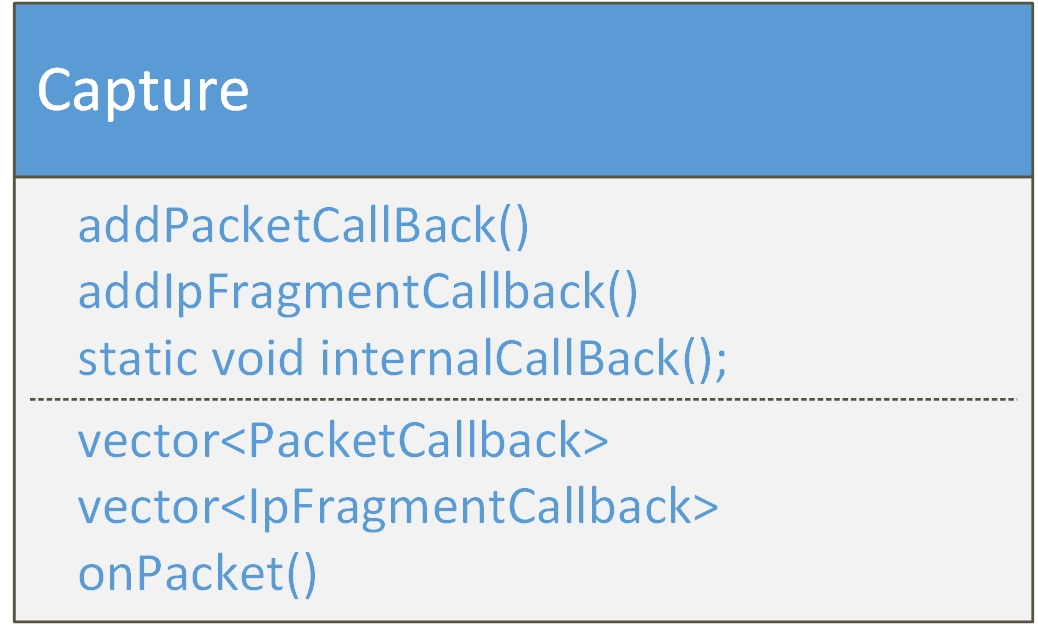
\includegraphics[width=0.25\textwidth]{./picture/Figure4.jpg}
  \caption{An Example of The Module}
  \label{fig:4}
\end{figure}

\section{Implementation}
We now give more details on the implementation of the noff monitoring framework.
\subsection{Multi-Thread}
Noff supports user-level multi-thread mechanism. Considering the compatibility of a network platform ,We offer two kinds of sharing scheme for programmers.The first one is built on NIC's RSS(receive-side scaling) scheme.
\newline\indent Multiple queue NICs provide multiple transmit and receive queues, allowing packets received by the NIC to be assigned to one of its receive queues. Each receive queue is assigned to a separate interrupt; by routing each of those interrupts to different cores. Processing of the interrupt requests triggered by the network traffic received by a single NIC can be distributed among multiple cores, bringing additional performance improvements in interrupt handling. Usually, a NIC distributes incoming traffic between the receive queues using a hash function.The first mechanism is accomplished through the PF\_RING driver.
\newline\indent The second multi-thread mechanism is built on user-level hash algorithm because some NICs may not support Multiple queues. In this scheme,a sharding module should compute the hash index for each captured packet which is in the light of the four tuples of this packet and then assigns it to the corresponding thread.The mapping of threads to CPU cores is likewise practically one-to-one.
\newline\indent Through the multi-thread mechanism, noff has advanced the runtime performance effectively.
\subsection{Powerful TCP Reassembly}
TCP reassembly is a resource-consuming procedure. Thus it is central to optimize this procedure. noff develops a new stream reassemble module based on Libnids.We then describe this from three aspects:
\subsubsection{Thread Safety}
Libnids' stream reassembly module is accomplished by C language and it has many global variables which may cause thread unsafety.Whereas noff's stream reassembly module is accomplished by C++ and all of the variables are capsulated which ensures that each thread is assigned an independent copy.
\subsubsection{Timing wheel}
The connection flood is a common network attack.If a TCP connection only has the SYN packets without the FIN packets,this connection will not be erased until the stream buffer size exceeds the threshold.In this case,the new stream may have no chance to be processed. Actually,a number of situations can finally cause this case. Libnids' reassembly engine has no ability to conquer with this circumstance.So referring to the current problems,noff adopts an innovative Keep-alive timer solution.Once a connection is established,the connection's keep-alive timer should be also established simultaneously.
\newline\indent In order to manage the timer effectively, we adopt a wheel like data structure\cite{Varghese} which can flexibly insert a new stream timer and erase a dead timer which has expired.A simple schematic diagram is given in Figure \ref{fig:5}. In this Figure there are totally seven time slots.Each slot represents one second and it is corresponding to a bucket which stores stream objects.When the system startups,the clock pointer should move to the next slot per second,Meanwhile the 0 slot would be dropped which means the stream objects in it also need to be dropped.And a new tail slot would be created.Through this way noff could knock out some dead streams.
\newline\indent noff need not only to knock out the dead streams but also to update the alive streams.In order to conveniently accomplish this function.we make use the reference count feature of the smart pointer.When we need to update a stream's timestamp,we just need to insert a shared\_ptr object of this stream into the current time slot bucket which means the reference count of this stream has an increment.When we drop a time slot bucket and the objects in it,only if a stream's reference count become zero,this stream could be erased from stream hash table drastically.Through this way,we can easily find out that we can just update a stream by just inserting a shared pointer of this stream.
\newline\indent Furthermore, through this mechanism,programmers can also set priority for one stream.A simple method is that they can update one stream continuously whether the stream has in exchange packets or not.
\newline\indent Noff uses circle queue to accomplish the wheel timer and set the number of the time slot to be 60 which means once a stream has no data in exchange for 60 seconds,it would become a dead stream and would be then erased.

\begin{figure}[htbp]
  \centering
  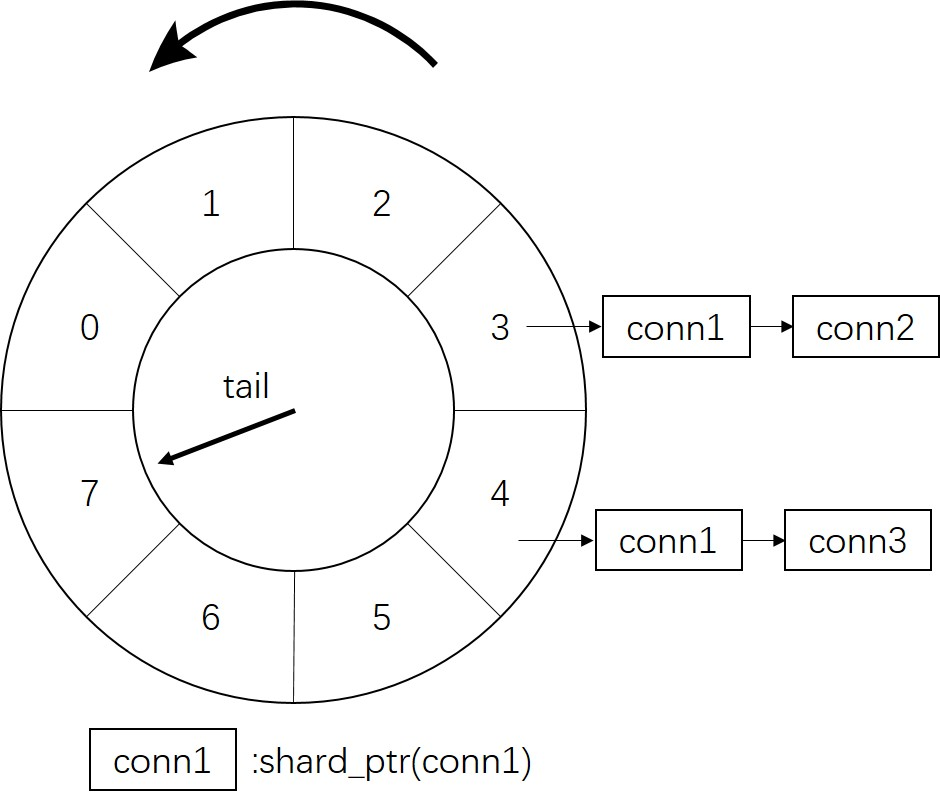
\includegraphics[width=0.25\textwidth]{./picture/Figure16.jpg}
  \caption{Schematic Diagram of Timing Wheel}
  \label{fig:5}
\end{figure}
\subsubsection{Memory Optimization}
The TCP reassembly module needs to resort TCP fragments.So it needs to prestore packet data which is meant by a large number of dynamic memory allocation. Libnids not only prestore packets but also store the completed packets between client and server. This scheme has a palpable short slab that there are too many memory allocations and copies which could bring huge overhead.
\newline\indent Basically, noff has abandon the scheme that the reassembly module needs to store the completed packets. Because though libnids offer this ability. The upper applications also have to store the TCP stream data by themselves again. After optimizing this procedure,the performance of stream reassembly module has been improved explicitly.
And further more,noff uses TCMalloc to optimize the memory allocation speed.
\subsection{Packets Filter and Statistic}
Noff has afforded three kinds of filters.The first one is PF\_RING filter,you should use \textbf{pfring\_add\_filter\_rule} function to add a filter rule on an existing ring.
The second one is BPF\_filter. BPF supports filtering packets, allowing a userspace process to supply a filter program that specifies which packets it wants to receive.
The third one is protocol filter which is embedded in Ip fragment module.It can filter the packets in the callback interface.Now it can filter packets according to registered module and port.For instance,TCP modules can use \textbf{registerRule} function to specify which packets they don't need.In this way,some packets may not be sent to the upper layer module again.So filters can increase the system performance to a certain extent.
\newline\indent Noff also provides much statistical information.Noff provides not only the basic kernel dropping information but also the number of processed packets in each filter and each thread.All of this information would be indicated through the system log. The following code block exhibits part of system log which lists the number of packets handled by each thread.
\begin{lstlisting}[language=C]
20170528 08:44:57.964400Z 128795 INFO
worker1: 7754 - Dispatcher.cc:48
20170528 08:44:57.964403Z 128795 INFO
worker2: 16902 - Dispatcher.cc:48
20170528 08:44:57.964405Z 128795 INFO
worker3: 20434 - Dispatcher.cc:48
\end{lstlisting}
\indent Our implementation is based on an intel 520 XR2 NIC and a BCM5720 NIC.The XR2 is a modern 10GbE NIC supporting multiple queues and RSS while the BCM5720 is a 1000MbE NIC which only supports single receive queue.Noff can be effectively used with both these NICs. Actually according to our test,Noff can be executed on nearly all NICs platform.

\subsection{Callback Interface}
Noff use C++ bind/function feature to actualize callback interface.Bind scheme generates a forwarding call wrapper for a member function of a class.Calling this wrapper is equivalent to invoking a member function with some of its arguments bound to args. 
All module classes in noff should register their member function through this way.Once one function has been registered in a module.This module would store it into a vector.When a specific event happens,all call wrappers in the vector should be invoked one by one.This scheme is described vividly in Figure \ref{fig:6}.
\newline\indent Actually this scheme is similar to Observer Pattern.
\begin{figure}[htbp]
  \centering
  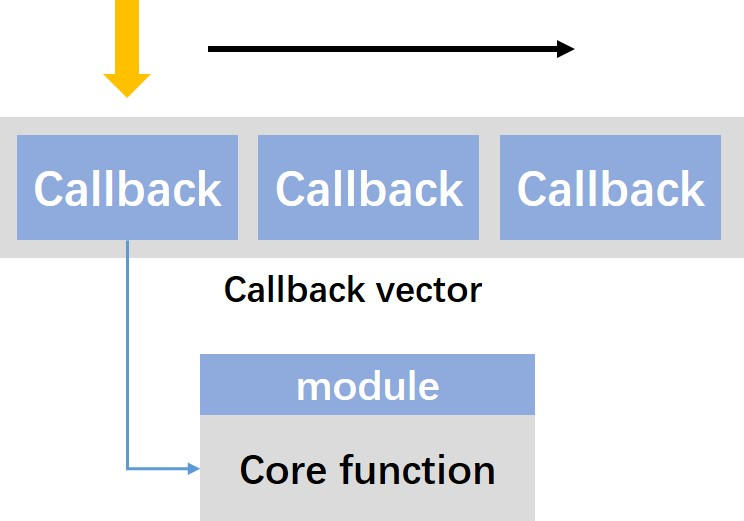
\includegraphics[width=0.3\textwidth]{./picture/Figure5.jpg}
  \caption{Callback Interface Scheme}
  \label{fig:6}
\end{figure}
\subsection{Packet Handle}
An application may be interested in receiving both reassembled streams, as well as their individual packets to detect TCP-level attacks.Different from traditional methods or to extract meritorious information from network traffic data. Because of callback interface in each module,noff's interfaces only offer necessary data for each module rather than delivering the original packets from the network.If an application indicates that it needs original data,in noff it needs to register with the capture module's interface.

\section{Experimental Evaluation}
We experimentally evaluate the performance and feature of noff, comparing it to other similar libraries, for common monitoring tasks, such as flow statistics export and http parser, while replaying a trace of real network traffic at different rates.

\subsection{Experimental Environment}

\subsubsection{Hardware}
In this paper,we use a testbed comprising two PCs interconnected directly through an Intel 520XR2 10GbE NIC and MT26448 10GbE NIC.Intel NIC is used as a stream capturer while MY26448 NIC is used for traffic generation. The two PCs are both equipped with one eight-core Intel Xeon 1.8GHz CPUs with 10MB L2 cache, 4GB RAM.Both PCs run 64-bit Ubuntu Linux(kernel version 4.4.50).
\begin{figure}
\begin{minipage}[t]{0.495\linewidth}
\flushleft
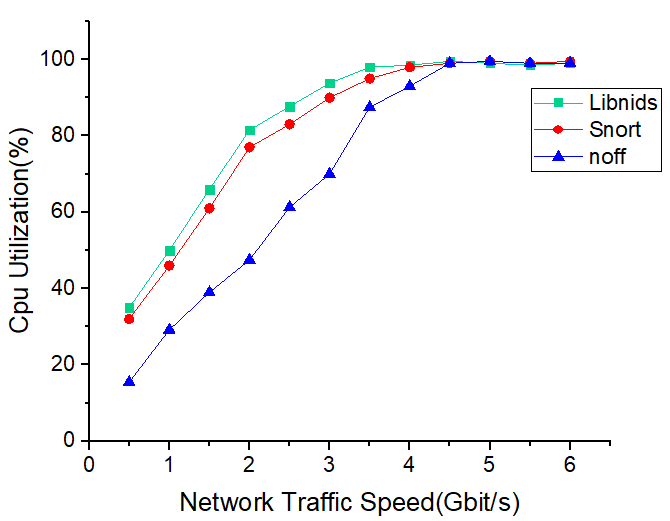
\includegraphics[width=\textwidth]{./picture/Figure6.jpg}
\caption{Packet loss} 
\label{fig:7}
\end{minipage}
\begin{minipage}[t]{0.495\linewidth}
\flushright
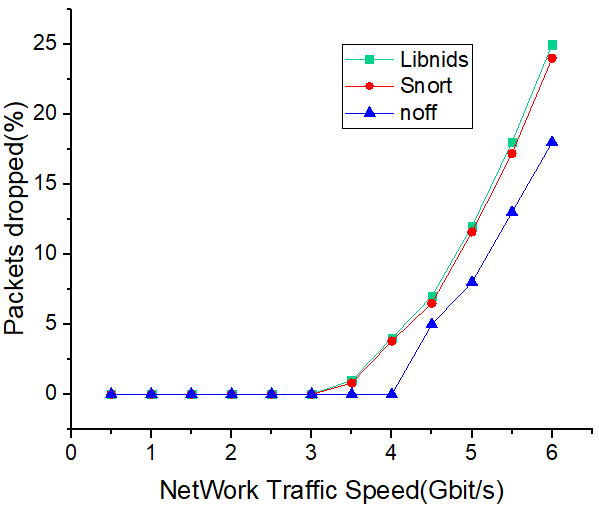
\includegraphics[width=\textwidth]{./picture/Figure7.jpg}
\caption{CPU Utilization}
\label{fig:8}
\end{minipage}
\end{figure} 
\subsubsection{Traffic}
To evaluate stream reassembly implementations with real traffic,we replay a traffic file which comes from campus network having totally two million TCP packets.
\subsubsection{Parameters}
We compare noff with the following libraries: (\uppercase\expandafter{\romannumeral1})Libnids v1.25\cite{Libnids}
(\uppercase\expandafter{\romannumeral2})and the Stream5 preprocessor of Snort v3.0.0. Libnids and Snort rely on Libpcap\cite{McCanne}, which uses the PF\_PACKET socket for packet capture on Linux while noff use PF\_PACKET directly .In our experiments, the size of this buffer is set to 512MB, and the buffer size for reassembled streams is set to 500000 for all of these three library.The other parameters for Libnids and Snort are all default.  
We set the keep-alive timer of noff as 60 seconds.As we replay the traffic data circularly,an inactivity timeout of 60 seconds is a reasonable choice.

\subsection{TCP Stream Processing Comparision}
The first experiment we evaluate the TCP stream reassemble performance of noff comparing with Snort Stream5 processor and a Libnids-based simple sniffer program that just receives reassembled streams.
In this experiment, noff only assembles TCP fragment module without advanced processing.Noff also drop UDP and ICMP packets directly.Similarly Libnids and Snort also drop all of them.When these libraries receive FIN or RST TCP packets,they just erase the entire TCP connection from hash table.For a fair comparison, we configure noff to only use a single worker thread, as Snort and Libnids are just single-threaded. And they all use PF\_RING as NIC driver.
\newline\indent Figures \ref{fig:7},Figure \ref{fig:8} present the percentage of dropped packets,the average Cpu utilizing of the monitoring application on a single core. We use the tool tcpreplay to replay the static network traffic at the rate from 500Mbit/s to 6Gbit/s.The result Figures indicate that The Libnids starts losing packets when the traffic rate exceeds 3Gbit/s. It is becasue that when the traffic rate exceeds 3Gbit/s, the CPU utilization of the Libnids exceeds 90\%. Also the Snort performs slightly better than Libnids,But it still start to losing packets when the traffic rate exceeds 3Gbit/s. At this time, the CPU utilization of the Snort also exceeds 90\%.Because the Snort and Libnids have similar stream processing schemes. 
\newline\indent Noff performs explicitly better than the Libnids and Snort.It starts to drop packets after the traffic rate exceeds 4Gbits/s.It is critical to figure that The Libnids,The Snort and the noff are all based on single-core PF\_RING driver.Which means that noff has better user-level optimization. In my opinion,the key optimization is the memory allocation.
\begin{figure}
\begin{minipage}[t]{0.495\linewidth}
\flushleft
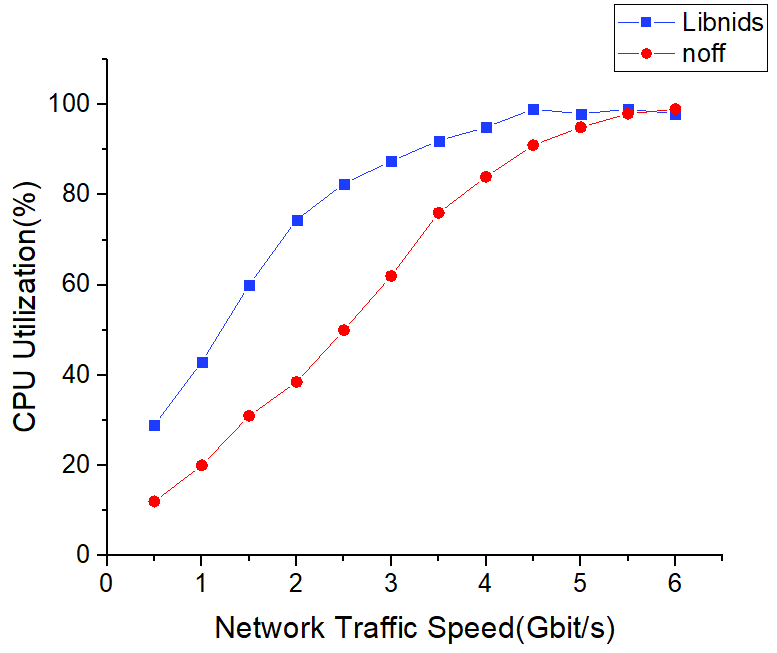
\includegraphics[width=\textwidth]{./picture/Figure8.jpg}
\caption{CPU Utilization of HTTP Parser} 
\label{fig:9}
\end{minipage}
\begin{minipage}[t]{0.495\linewidth}
\flushright
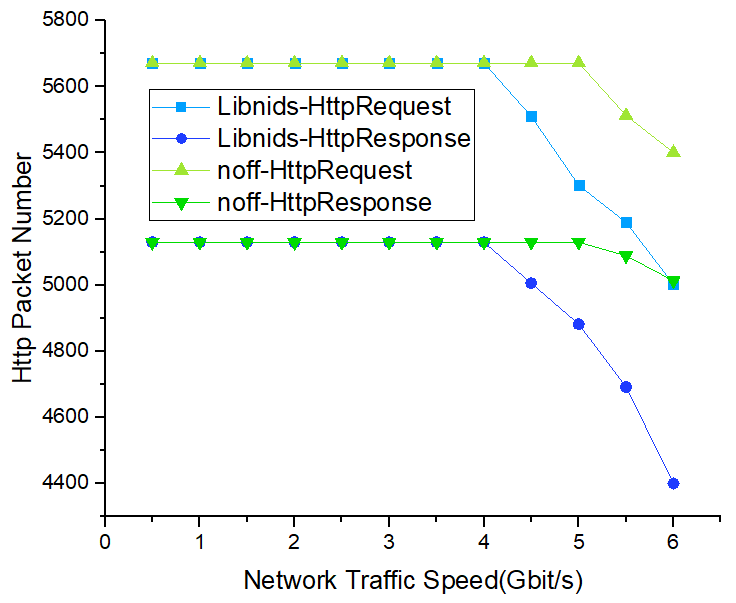
\includegraphics[width=\textwidth]{./picture/Figure9.jpg}
\caption{Http Packet Number}
\label{fig:10}
\end{minipage}
\end{figure} 
\subsection{Http Information Processing Comparision}
The second experiment is involved with the application of noff. The Hypertext Transfer Protocol (HTTP) is an application protocol for distributed, collaborative, and hypermedia information systems. HTTP is the foundation of data communication for the World Wide Web. In this experiment,We have separately developed a HTTP parser application module for the three library(noff,Libnids,Snort).the modules collect HTTP data from TCP layer then extract critical information from the headers of HTTP packets and finally export the statistic information for each HTTP connection.
\newline\indent The procedure of HTTP parsing is shown as this:The module firstly collects the TCP streams which have been reassembled.Then the module filters the useless streams through port matching.
And then the module should put the TCP data into a http parser tool to obtain the HTTP header's information.
\newline\indent In this experiment, we evaluate the performance of parsing HTTP packets of noff comparing with the Libnids which has assembled the same HTTP module as noff.In order to acquire relatively stable experimental results. We use a static TCP streams dataset from SJTU campus.All of TCP packets' port in this dataset are all 80 and there are totally 5672 HTTP request packets and 5130 HTTP response packets. Figure \ref{fig:9} and Figure \ref{fig:10} indicate the average CPU utilization of the monitoring application on a single core,and the HTTP packets number statistic information on a single core while varying the traffic rate from 500Mbit/s to 6Gbit/s.We see that Libnids starts losing 
HTTP packets when the traffic rate exceeds 4Gbit/s. The reason can be seen in Figure \ref{fig:9},where the total CPU utilization of Libnids exceeds 90\% at 4Gbit/s.Meanwhile,noff starts to drop HTTP packets at 5Gbit/s.Comparing the experiment of TCP reassembly, we can find that the performance of noff application is also better than Libnids.
\begin{figure}
\begin{minipage}[t]{0.495\linewidth}
\flushleft
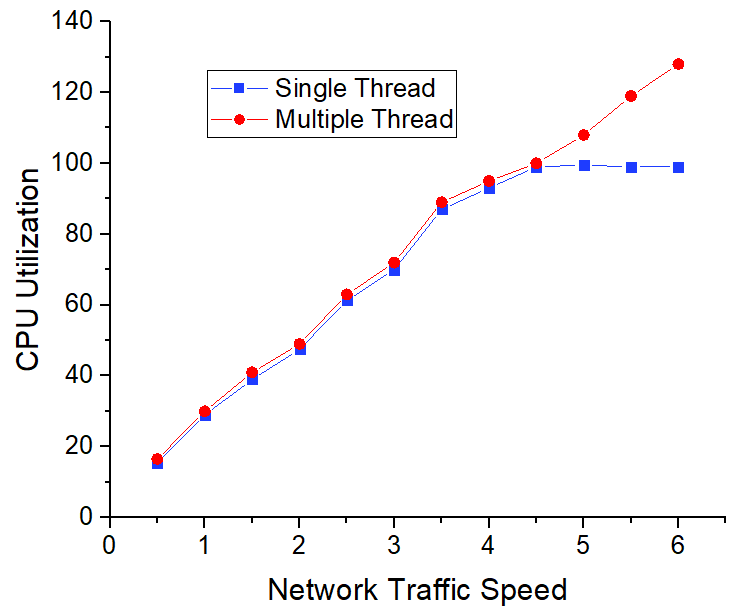
\includegraphics[width=\textwidth]{./picture/Figure10.jpg}
\caption{CPU Utilization of Single and Multiple Thread} 
\label{fig:11}
\end{minipage}
\begin{minipage}[t]{0.495\linewidth}
\flushright
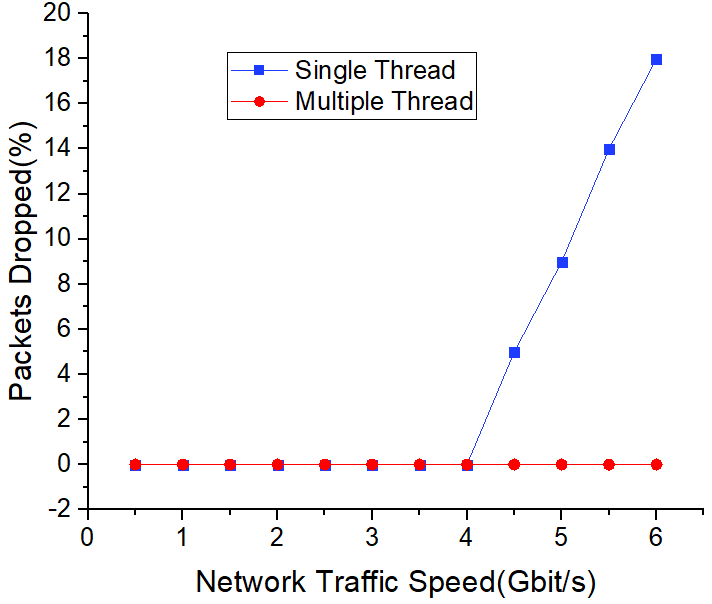
\includegraphics[width=\textwidth]{./picture/Figure11.jpg}
\caption{Packet Loss of Single and Multiple Thread}
\label{fig:12}
\end{minipage}
\end{figure} 
\subsection{Multiple Thread and Multiple Core}
In the Implementation section,we declare that the PF\_RING driver can support multiple queue NIC packet capture. In this experiment,we should verify the value of multiple thread.
\newline\indent Our 10GBE NIC can support 8 receive queues. So we would compare the performance of noff's TCP reassemble on single thread with the performance on multiple thread. Actually, multiple thread does not bring too much additional overhead.Each thread should burden the same procedure. Through NIC's RSS,each thread would only process one-eighth streams compared with the single thread scheme.
\newline\indent The Figure \ref{fig:11} and Figure \ref{fig:12} indicate the experiment result which include the performance of noff on two cases.From the result, we can clearly see that the single thread case starts to drop packets when the traffic rate exceeds 4Gbit/s while the multiple thread case drops no packet even the the traffic rate exceeds 6Gbit/s.We can find the reason from \ref{fig:11}.when the traffic rate exceeds 4Gbit/s,the single core utilization arrives the threshold(100\%) which means noff arrives its limitation on single core.But on multiple core platform,noff can use several cores to improve its processing ability.The utilization of it can exceed 100\%.This experiment prove that by multiple thread scheme,noff can obtain better performance extremely.
\newline\indent In the implementation section, we also refer an user-level multiple thread scheme.Different from the RSS method.The user-level method has an extra memory copy and brings a synchronization Lock.So the user-level multiple thread can not always improve performance.According to our experiment,when the work per thread is too heavy,the user-level multiple thread may become a better choice. 

\subsection{TCMalloc Optimization}
Memory copy always bring remarkable influence to performance.In this paper we adopt the TCMalloc tool to accelerate the memory copy process.In this experiment, we 
would compare the noff's performance in the two cases:with TCMalloc and without TCMalloc.In order to control the variables,we decide to reuse the test scenario in TCP stream reassembly experiment.
\newline\indent The Figure \ref{fig:13} and Figure \ref{fig:14} indicate the result of experiment.From the Figure \ref{fig:13},we can see that the CPU utilization is slightly higher when we don't use TCMalloc. So the consequence is that when we don't use TCMalloc noff starts to drop packets when the network traffic exceeds 3.5Gbit/s.This check experiment prove that TCMalloc can improve the memory copy performance to a certain extent.
\newline\indent The full name of TCMalloc is thread cache malloc. One of the key  exploring spots is the thread local cache. In multiple thread environment,noff's module classes are all thread cache variables. So In this environment,the TCMalloc tool is a much better memory allocation optimization method.
\begin{figure}
\begin{minipage}[t]{0.495\linewidth}
\flushleft
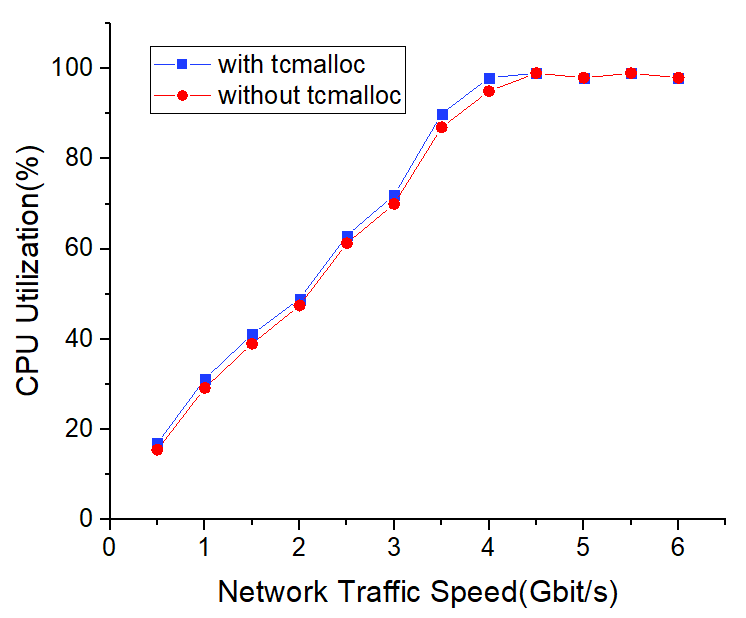
\includegraphics[width=\textwidth]{./picture/Figure12.jpg}
\caption{CPU Utilization with TCMalloc or not} 
\label{fig:13}
\end{minipage}
\begin{minipage}[t]{0.495\linewidth}
\flushright
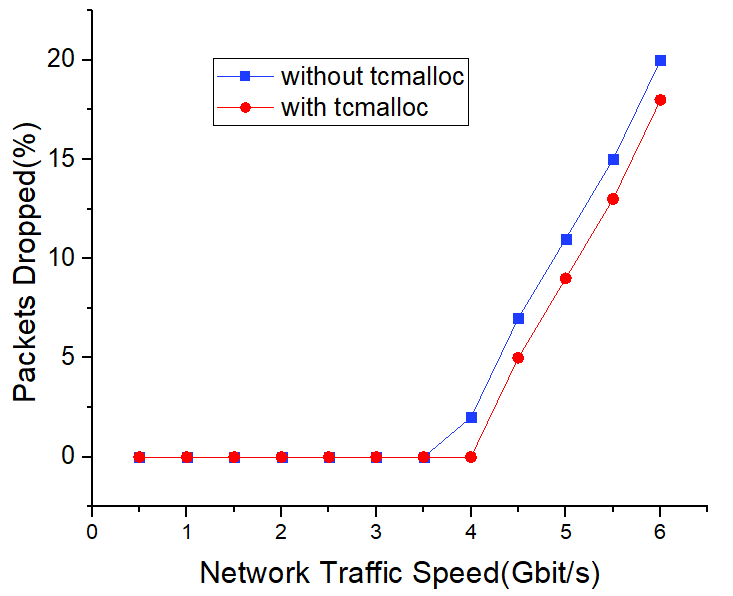
\includegraphics[width=\textwidth]{./picture/Figure13.jpg}
\caption{Packet Loss with TCMalloc or not}
\label{fig:14}
\end{minipage}
\end{figure} 

\subsection{Concurrent Traffic}
In the previous section,we have involved the Least Recently Used algorithm implementation and timing wheel scheme to manage the stream hash table.In this experiment, we need to confirm the effectiveness of these two methods.In order to attain the objective, we hope to verify this system from two aspects: multiple concurrent traffic processing and the no FIN streams processing.
\newline\indent For the first aspects,we use a real network TCP traffic set from SJTU campus network as the test data.In this set,there are totally about 50000 streams.We would vary the size of stream hash table of noff and libnids from 500 to 30000.Then record the number of loss streams of libnids and noff.
The figure \ref{fig:15} indicates the result of experiment.From the figure,we can explicitly see that libnids drops more streams than noff under the same circumstances. Actually these two library would eventually drop about 4000 streams when they have plenitudinous table size. 
\newline\indent For the second aspects,we have imitated multiple streams. These streams are all no FIN packets.In this way, if the capture library has no scheme to erase the dead streams.The streams would take up one position of 
the table.Noff can use time wheel to kick away the dead streams.So it should have a better performance in this situation.The figure \ref{fig:16} indicates the result of this experiment.we imitate the no FIN stream at the speed of 10Mbit/s and compare the number of loss stream of noff and libnids from 10s to 
120s.From the figure \ref{fig:16} we can see that noff and libnids have similar performance before 60s while noff obviously drop less packets after 60s for that noff's keep-alive timer works.The timer drops the dead stream from stream table.
\newline\indent Through these two experiments,we can reach the conclusion that noff has a better stream manager scheme.It can process multiple streams more flexibility.
\begin{figure}
\begin{minipage}[t]{0.49\linewidth}
\flushleft
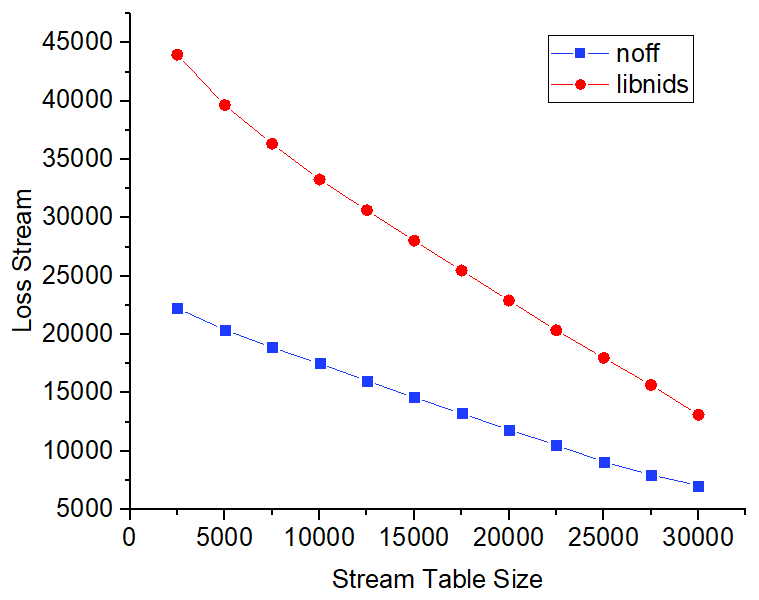
\includegraphics[width=\textwidth]{./picture/Figure14.jpg}
\caption{Stream Loss with Different Hash Table Size} 
\label{fig:15}
\end{minipage}
\begin{minipage}[t]{0.49\linewidth}
\flushright
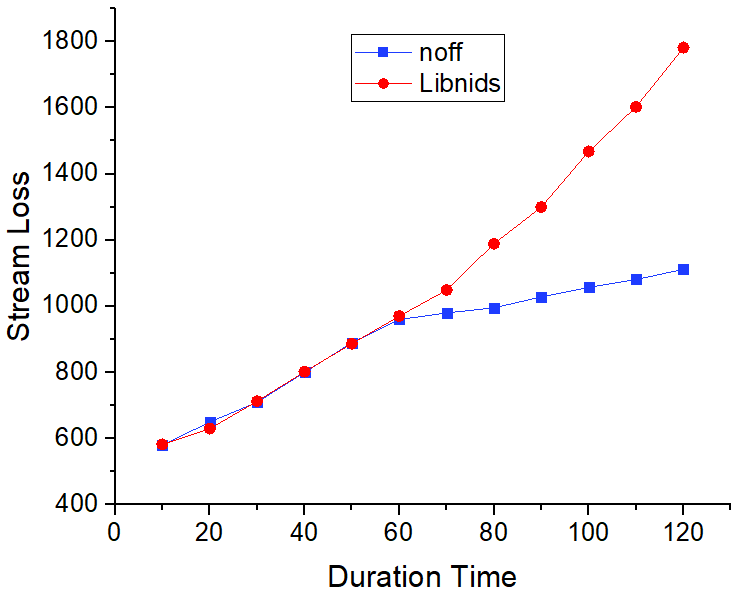
\includegraphics[width=\textwidth]{./picture/Figure15.jpg}
\caption{Stream Loss with Different Duration}
\label{fig:16}
\end{minipage}
\end{figure} 







% An example of a floating figure using the graphicx package.
% Note that \label must occur AFTER (or within) \caption.
% For figures, \caption should occur after the \includegraphics.
% Note that IEEEtran v1.7 and later has special internal code that
% is designed to preserve the operation of \label within \caption
% even when the captionsoff option is in effect. However, because
% of issues like this, it may be the safest practice to put all your
% \label just after \caption rather than within \caption{}.
%
% Reminder: the "draftcls" or "draftclsnofoot", not "draft", class
% option should be used if it is desired that the figures are to be
% displayed while in draft mode.
%
%\begin{figure}[!t]
%\centering
%\includegraphics[width=2.5in]{myfigure}
% where an .eps filename suffix will be assumed under latex, 
% and a .pdf suffix will be assumed for pdflatex; or what has been declared
% via \DeclareGraphicsExtensions.
%\caption{Simulation results for the network.}
%\label{fig_sim}
%\end{figure}

% Note that the IEEE typically puts floats only at the top, even when this
% results in a large percentage of a column being occupied by floats.


% An example of a double column floating figure using two subfigures.
% (The subfig.sty package must be loaded for this to work.)
% The subfigure \label commands are set within each subfloat command,
% and the \label for the overall figure must come after \caption.
% \hfil is used as a separator to get equal spacing.
% Watch out that the combined width of all the subfigures on a 
% line do not exceed the text width or a line break will occur.
%
%\begin{figure*}[!t]
%\centering
%\subfloat[Case I]{\includegraphics[width=2.5in]{box}%
%\label{fig_first_case}}
%\hfil
%\subfloat[Case II]{\includegraphics[width=2.5in]{box}%
%\label{fig_second_case}}
%\caption{Simulation results for the network.}
%\label{fig_sim}
%\end{figure*}
%
% Note that often IEEE papers with subfigures do not employ subfigure
% captions (using the optional argument to \subfloat[]), but instead will
% reference/describe all of them (a), (b), etc., within the main caption.
% Be aware that for subfig.sty to generate the (a), (b), etc., subfigure
% labels, the optional argument to \subfloat must be present. If a
% subcaption is not desired, just leave its contents blank,
% e.g., \subfloat[].


% An example of a floating table. Note that, for IEEE style tables, the
% \caption command should come BEFORE the table and, given that table
% captions serve much like titles, are usually capitalized except for words
% such as a, an, and, as, at, but, by, for, in, nor, of, on, or, the, to
% and up, which are usually not capitalized unless they are the first or
% last word of the caption. Table text will default to \footnotesize as
% the IEEE normally uses this smaller font for tables.
% The \label must come after \caption as always.
%
%\begin{table}[!t]
%% increase table row spacing, adjust to taste
%\renewcommand{\arraystretch}{1.3}
% if using array.sty, it might be a good idea to tweak the value of
% \extrarowheight as needed to properly center the text within the cells
%\caption{An Example of a Table}
%\label{table_example}
%\centering
%% Some packages, such as MDW tools, offer better commands for making tables
%% than the plain LaTeX2e tabular which is used here.
%\begin{tabular}{|c||c|}
%\hline
%One & Two\\
%\hline
%Three & Four\\
%\hline
%\end{tabular}
%\end{table}


% Note that the IEEE does not put floats in the very first column
% - or typically anywhere on the first page for that matter. Also,
% in-text middle ("here") positioning is typically not used, but it
% is allowed and encouraged for Computer Society conferences (but
% not Computer Society journals). Most IEEE journals/conferences use
% top floats exclusively. 
% Note that, LaTeX2e, unlike IEEE journals/conferences, places
% footnotes above bottom floats. This can be corrected via the
% \fnbelowfloat command of the stfloats package.

\section{Related Work}
In this section, we would introduce some previous related work of other researchers.

\subsection{Kernel Capture Optimization}
Scap\cite{Papadogiannakis} is a novel capture library whose most attractive distinguishing characteristic is that it offer a NIC driver to process packet data in multiple receive queue.Its modules are mainly deployed in kernel level which means it has an aggressive performance.And scap also provide some  meticulous system optimization method.To tell the truth,scap is actually an excellent research work. By contrast, noff directly use PF\_RING driver to accomplish the similar function.But noff also support an user-level multiple thread platform to enhancing the versatility of the library.After all,not all NIC support multiple receive queue.

\subsection{Multicore Architecture}
Multicore architecture creates a new epoch in research on parallel processing.Many researches have been done.For example Low-level CPU optimizations like those of
L2-cache is one practical solution for fast parallelization\cite{Zhanikeev} and Chen et al. \cite{MapReduce} perform parallel processing of Big Data but optimize resource use.Marat Zhanikeev\cite{Zhanikeev} proposed a lockfree method to speed up capture process.Scap\cite{Papadogiannakis} is another kernel-level based optimization method and Schultz\cite{Schultz} claims that baremetal can handle the 10Gbps traffic on a single core.Noff adopt a lockfree user-level multi-thread platform.
\subsection{TCP Stream Reassembly}
Libnids\cite{Libnids} and Stream5\cite{Sturges} perform TCP reassembly based on the emulation of a network stack. Noff propose a more high-performance reassembly engine which optimize the drawbacks of libnids.


\subsection{Structure Optimization}
Luca Deri\cite{Deri} proposed a method based on polling frame to optimize the packets processing procedure.Yeim-Kuan\cite{Chang} make use of hierarchical binary prefix search scheme to process packets.Noff uses flexible callback interfaces to help programmers to build flexible structure easily.


\section{Conclusion}
In this paper,we have analyzed the significance in capturing and parsing the completed traffic network stream. So a high-performance capture traffic is badly demanded.Actually most programmers need a high-Performance capture as well as a flexible extendible library to add some aggressive applications.To cope with this conundrum. We have proposed our work:noff which is a flexible high-performance network traffic capture library.It has both kernel-level and user-level based multi-thread scheme to adapt to nearly all kinds of NICs.And it offers many flexible callback interfaces to help programmers to organise the system framework effectively.Compared with existing library libnids, noff has Imposed a variety of optimization such as memory allocation,TCP reassembly and so on.In this paper we evaluate our implementation through several experiments.
\newline\indent The results of our experimental evaluation demonstrate that noff can  capture network traffic for speed up to 4Gbit/s without packets loss using a single core which is better than the other existing approaches.A HTTP parsing application based on noff's platform is also performed better than the the other existing approaches.Moreover,noff support multi-thread,using this scheme noff can cope with the network traffic whose speed is up to 6Gbit/s easily.Meanwhile,noff's stream management algorithm help it to drop nearly 50\% fewer streams than the existing approaches when facing the high concurrence traffic.We can also build a new application based on noff faster.
\newline\indent We believe our implementation can bring some novel idea for developing an
attractive network library. 



% conference papers do not normally have an appendix


% use section* for acknowledgment
\section*{Acknowledgment}

We would like to thank the junior student Guangqian Peng.He has offered a huge contribution to this research work.This research was performed with the financial support from an industrial project. The experts of SJTU also have been involved in this project and offered some valuable feedback.





% trigger a \newpage just before the given reference
% number - used to balance the columns on the last page
% adjust value as needed - may need to be readjusted if
% the document is modified later
%\IEEEtriggeratref{8}
% The "triggered" command can be changed if desired:
%\IEEEtriggercmd{\enlargethispage{-5in}}

% references section

% can use a bibliography generated by BibTeX as a .bbl file
% BibTeX documentation can be easily obtained at:
% http://mirror.ctan.org/biblio/bibtex/contrib/doc/
% The IEEEtran BibTeX style support page is at:
% http://www.michaelshell.org/tex/ieeetran/bibtex/
%\bibliographystyle{IEEEtran}
% argument is your BibTeX string definitions and bibliography database(s)
%\bibliography{IEEEabrv,../bib/paper}
%
% <OR> manually copy in the resultant .bbl file
% set second argument of \begin to the number of references
% (used to reserve space for the reference number labels box)
\begin{thebibliography}{1}

  \bibitem{Liu}
  Liu, Duo, et al. "High-performance packet classification algorithm for many-core and multithreaded network processor." International Conference on Compilers, Architecture and Synthesis for Embedded Systems ACM, 2006:334-344.
  
  \bibitem{Antonello}
  Antonello, Rafael, et al. "Deep packet inspection tools and techniques in commodity platforms: Challenges and trends." Journal of Network \& Computer Applications 35.6(2012):1863-1878.
  
  \bibitem{Qiao}
  Qiao, Siyi, et al. "Network recorder and player: FPGA-based network traffic capture and replay." International Conference on Field-Programmable Technology IEEE, 2015.
  
  \bibitem{Ali}
  Ali, Sardar, et al. "On mitigating sampling-induced accuracy loss in traffic anomaly detection systems." ACM SIGCOMM Computer Communication Review 40.3(2010):4-16.
  
  \bibitem{PFRING}
  PF\_RING. http://www.ntop.org/products/packet-capture/pf\_ring/
  
  \bibitem{Luca}
  Luca Deri, “Modern Packet Capture and Analysis: Multi-Core, Multi-
Gigabit, and Beyond”, Internet Measurement (IM) Tutorial, 2009.

  \bibitem{snort}
  Sourcefire vulnerability research team (vrt). http://www.
snort.org/vrt/.

  \bibitem{Evans}
  J. Evans. Scalable memory allocation using jemalloc. 2011. http://www.facebook.com/notes/facebook-engineering/scalable-memory-allocation-using-jemalloc/480222803919.
  
  \bibitem{Threading}
  Intel Threading Building Blocks. https://software.intel.com/en-us/intel-tbb/
  
  \bibitem{Sangho}
  Lee, Sangho, T. Johnson, and E. Raman. "Feedback directed optimization of TCMalloc." The Workshop on Memory Systems PERFORMANCE and Correctness ACM, 2014:3.
  
  \bibitem{Server}
  Intel Server Adapters. Receive Side Scaling on Intel Network Adapters. http://www.intel.com/support/network/adapter/pro100/sb/cs-027574.htm.
  
  \bibitem{Varghese}
  Varghese, G., and A. Lauck. "Hashed and hierarchical timing wheels: efficient data structures for implementing a timer facility." IEEE/ACM Transactions on Networking 5.6(2002):824-834.
  
  \bibitem{Libnids}
  Libnids. http://libnids.sourceforge.net/.
  
  \bibitem{Papadogiannakis}
  Papadogiannakis, Antonis, M. Polychronakis, and E. P. Markatos. "Scap: stream-oriented network traffic capture and analysis for high-speed networks." Conference on Internet Measurement Conference ACM, 2013:441-454.
  
  \bibitem{McCanne}
  S. McCanne, C. Leres, and V. Jacobson. Libpcap. http://www.tcpdump.org/. Lawrence Berkeley Laboratory.
  
  \bibitem{Machdi}
  Machdi, Imam, T. Amagasa, and H. Kitagawa. "Executing parallel TwigStack algorithm on a multi-core system." International Conference on Information Integration and Web-Based Applications \& Services ACM, 2009:176-184.
  
  \bibitem{Zhanikeev}
  Zhanikeev, Marat. A lockfree shared memory design for high-throughput multicore packet traffic capture. Wiley-Interscience, 2014.
  
  \bibitem{MapReduce}
  Chen R, Chen H, Zang B. Tiled-MapReduce: optimizing resource usages of data-parallel applications on multicore with tiling. In 19th International Conference on Parallel Architectures and Compilation Techniques (PACT), 2010;523–534.
 
  
  \bibitem{Sturges}
  J. Novak and S. Sturges. Target-Based TCP Stream Reassembly. http://assets.sourcefire.com/snort/developmentpapers/stream5-model-Aug032007.pdf, 2007.
  
  \bibitem{Deri}
  L Deri,NSPA Via,B Km,LL Figuretta.Improving passive packet capture: beyond device polling.Proceedings of Sane;2004.
  
  \bibitem{Chang}
  Chang, Yeim Kuan, and F. C. Kuo. "Towards optimized packet processing for multithreaded network processor." International Conference on High PERFORMANCE Switching and Routing IEEE, 2010:127-132.
  
  \bibitem{Schultz}
  Schultz, Michael J., and P. Crowley. "Performance Analysis of Packet Capture Methods in a 10 Gbps Virtualized Environment." International Conference on Computer Communications and Networks IEEE, 2012:1-8.
  
  
\end{thebibliography}



% that's all folks
\end{document}


